\section{Etat de l'art}
\noindent
Nous venons de présenter le fonctionnement d'une simple structure de données pour les maillages tétraèdriques. Elle ne peut pas être considérée comme compacte car elle utilise trop de références. Nous allons dans cette partie nous intéresser aux algorithmes de compression et structures de données compactes pour les maillages surfaciques et volumiques. Bien que notre travail soit uniquement centré sur les maillages volumiques, l'essentiel des travaux effectués jusqu'à présent est consacré aux maillages surfaciques.\\
Que ce soit pour de la compression ou pour une structure de données compacte, on peut réduire la taille mémoire d'un maillage en le simplifiant (supprimer des sommets...), en encodant la géométrie et/ou la connectivité du maillage. Nous ne nous intéresserons ici qu'à la réduction de la taille de la connectivité puisque c'est la plus gourmande en mémoire.\\
%Les maillages sont la pluspart du temps stockés sous forme indexés. Dans un premiers temps, on énumère pour chaque sommet ses coordonnées géométriques. 
%Puis pour chaque face (resp. tétraèdre), les indices de ses 3 (resp. 4) sommets. D'autres attributs peuvent être stockés (normales, couleurs...) mais nous n'en discuterons pas ici. Les formats indexés ne sont pas les formats les plus concis pour sauvegarder des maillages. En effet, la connectivité occupe une place très importante. Tandis que dans les maillages triangulaires surfaciques, le degré moyen d'un sommet est 6, il est de 22 dans les maillages tétraèdriques. Par conséquent, dans ce type de format, un sommet apparaitra dans 22 tétraèdres différents.\\
%La compression de maillages peut être séparer en 3 catégories : simplification polyhedrale, compression de positions, compression des informations de connectivités.\\\\
%\textbf{La simplification polyhedrale} consiste à simplifier le maillages en réduisant le nombre de sommets et en modifiant leurs positions afin que le nouveaux maillages reste aussi proche que possible de l'ancien. Ce sont des compression de maillages avec perte et ne sont donc pas adaptés aux usages nécessitant le maillage exact.\\\\
%\textbf{Compression des positions}\\\\
%\textbf{Compression de la connectivite}. La compression des informations de connectivité permet de réduire la redondance d'informations d'adjacence entre les k-simplexe d'un k-objet.\\\\
%En effet, comme dit dans la première partie, la structure de données doit être capable de répondre à des requetes simples (ex: donner les tetras adjacents à un tetra). Sans compression, cela signifie que chaque tetra doit stocker 4 références vers ses 4 tetras voisins. De plus, si l'on veut connaître les sommets composants un tetra, il est nécessaire de sauvegarder 4 references vers les 4 sommets composant le tetra. Ainsi, nous avons 8 références par tetra. Par conséquent, dans un maillage contenant 10000 tetras et en utilisant des références sur 32 bits, nous utiliserions 10000*8*32=2mo de références.
%On distingue les algorithmes de compression de maillages des structure de données pour maillages. Les premiers tentent de limiter au maximum l'usage mémoire du maillage en compressant le maillage. Le maillage devient inutilisable sous forme compressé, il est nécessaire de le décompresser pour l'utiliser à nouveau. En revanche, la structure de données pré-traite le maillage mais le maillage reste utilisable sous forme compressé.\\
La mesure utilisée pour évaluer la qualité d'une compression est le nombre de bits par sommets (bits per vertex ou bpv) tandis que la mesure utilisée pour évaluer la qualité d'une structure de données compacte est le nombre de références par triangle (resp. tétraèdre) rpt pour les maillages surfaciques (resp. volumiques).
\subsection{Maillages 2D}
\subsubsection{Compression}
\noindent
\textbf{Bande de triangles}. Les bandes de triangles ("triangles strips") et les eventails de triangles ("triangle fans") sont des représentations utilisées pour transférer les maillages de la mémoire centrale du PC vers la mémoire du GPU. Une bande de triangles est une séquence de sommets où chaque nouveau sommet défini un triangle avec les deux précedent sommets. En ce qui concerne les bandes de triangles, le but est de trouver de très longues bandes. Si celles-ci sont suffisamment longues alors, cette représentation permet de passer de 3N références aux sommets à N+2. L'algorithme de Deering utilise ces bandes de triangles et utilise entre 3.3 et 9.8 bpv \cite{triangle_strips}.\\
\textbf{Traversée de triangles}. La Cut border Machine \cite{cut_border_machine_2d} est un algorithme de Gumhold qui encode la connectivité en parcourant le graphe en largeur. L'algorithme étend la frontière défini par un triangle initial en traversant itérativement des triangles adjacents. Sept symboles sont utilisés pour préciser si la frontière a été étendue en insérant un nouveau sommet, si la frontière a été séparée ou si deux frontières se sont jointes. Le schéma peut compresser des variétés avec 4 bpv. En revanche, ce résultat est seulement valide pour des maillages réguliers. En effet, quand une jointure est effectuée, un décallage doit être fait pour désigner les sommets concernés. Par conséquent, il n'y a pas de borne supérieure garantie pour la compression avec cet algorithme.\\
L'algorithme EdgeBreaker de Rossignac \cite{edgebreaker} traverse lui aussi le graphe d'un triangle adjacent à un autre et enregistre la connectivité d'un maillage en produisant les sympboles C,L,R,E,S. Cependant, il garantit un coût de 4bpv.\\
\textbf{Codage de la Valence}. Une manière de décrire la connectivité des sommets est à travers leur valence. Le premier travail sur la valence des sommets est le travail de Touma et Gotsman \cite{valence_encoding}. Le principe est de considérer la frontière d'un triangle initial et de l'étendre en ajoutant itérativement de nouveaux sommets. La connectivité est encodée en utilisant la valence des nouveaux sommets (concentrée autour de 6). Ainsi, la liste de valences des sommets peut être efficacement compressée par un encodeur d'entropie (2.3 bpv). C'est toujours aujourd'hui l'une des méthodes les plus efficace.
\subsubsection{Structure de données compacte}
\noindent
Plusieurs structures de données permettent une utilisation très facile des maillages et se focalisent sur l'utilisation des arêtes du graphe. C'est le cas d'Half-Edge, Winged-Edge \cite{winged_edge} et Quad-Edge qui stockent $19n$ références (soit 9.5 rpt). Elles permettent facilement de naviguer dans le maillage et opèrent des requêtes d'adjacence en temps constant. Cependant, elles occupent trop de place pour être considérées comme compactes.\\
La Corner Table (CT) est à la base de plusieurs structures de données. Elle utilise deux listes V et O de $3|F|$ entiers chacune où $F$ est l'ensemble des faces du maillage. La table V stocke les incidences triangle/sommet tel-que les 3 sommets bordant un triangle t sont consécutifs (V[3t],V[3t+1],V[3t+2]) et sont listés dans un ordre consistent avec le maillage. Ainsi, V[c] représente un coin c associé avec une face f et un sommet. La table O stocke la référence entière du coin oposé. Le coin opposé o(c) au coin c est un coin dans un triangle adjacent qui partage la même arête opposée.\\
\begin{figure}[H]
\begin{center}
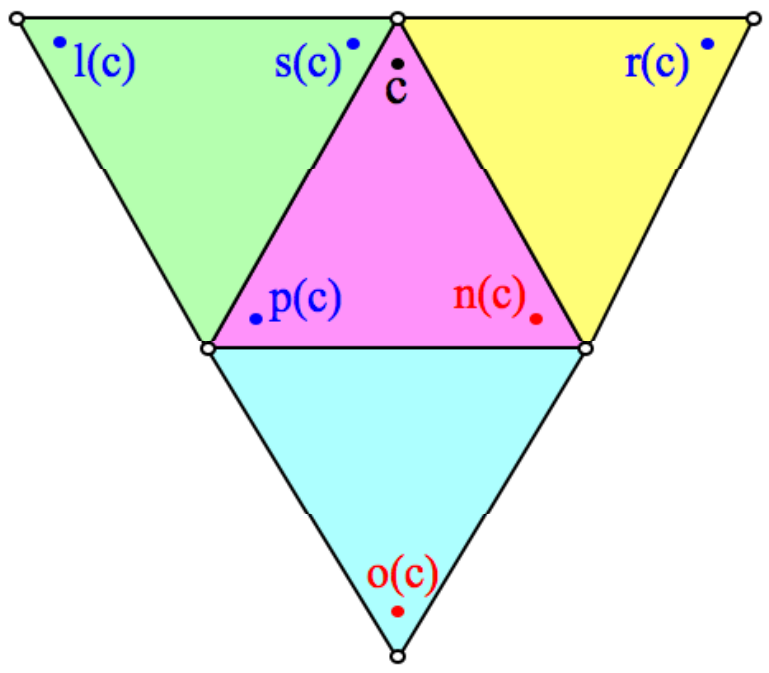
\includegraphics[scale=0.13]{Images/corner_table}
\caption{Les opérateurs utilisant les coins pour un maillage triangulaire}
\label{fig:corner_table}
\end{center}
\end{figure}
\noindent\ignorespacesafterend
\textbf{VOT}. La structure de données VOT (Vertex Opposite Table) est la première structure de données à utiliser cette 'Corner Table'. Elle permet une répresentation simple et efficace des maillages avec 6 références par triangle (3 références pour les sommets dans la table V et 3 références pour les coins dans la table O).\\
\textbf{SOT}. Développée par Rossignac \cite{SOT} est une amélioration de VOT où la table O est réordonnée et la table V supprimée. Néanmoins, l'accès au coin d'un sommet et à l'étoile d'un sommet sont toujours en temps constant. Cette dernière structure de données utilise 3 rpt en moyenne.\\
\textbf{SQUAD}. Dans SQUAD \cite{squad}, les auteurs traversent le graphe en prodondeur afin d'appareiller les triangles deux à deux avec l'un de leurs sommets partagés. Cela leur permet d'avoir 4 références par quad (i.e paire de triangles) et donc d'économiser une référence par triangle\footnote{Ils ne stockent pas la relation d'adjacence entre les deux triangles du même quad}. Quant aux triangles non appareillés, ils sont déguisés comme des quads. D'autre part, tout comme SOT, ils utilisent l'ordre des quads tel-que le ième quad soit associé au ième sommet. Dans un maillage surfacique, il y a deux fois plus de triangles que de sommets (cf. \ref{combi_2d}). Par conséquent, le nombre de quads et le nombres de sommets devrait être assez proche. Leur structure utilise en moyenne 2 rpt.
\begin{table}[H]
\centering
\footnotesize
\begin{tabular}{|c | c | c | c | c|}
\hline
Structure de données & Taille mémoire & Temps de navigation & Accès au sommet & Dynamique\\
\hline
Basées sur les arêtes & \multirow{2}{*}{18n+n} & \multirow{2}{*}{O(1)} & \multirow{2}{*}{O(1)} &\multirow{2}{*}{oui}\\
(Half-edge, Quad-edge, Winged-edge)&&&&\\
Basées sur les triangles & 13n & O(1) & O(1) & oui\\		
Corner table & 13n & O(1) & O(1) & oui\\
\hline
2D catalog \cite{2d_catalog}& 7.67n & O(1) & O(1) & oui\\
\hline
Star vertices \cite{star_vertices} & 7n & O(d) & O(1) & non\\		
SOT \cite{SOT}& 6n & O(1) & O(d) & non\\
SQUAD \cite{squad}& $(4+\epsilon)$n & O(1) & O(d) & non\\
%LR & $(2+\delta)$n & O(1) & O(d) & non\\
\hline  
\end{tabular}
\caption{Taille mémoire et performances des structures de données pour maillages surfaciques. n représente le nombe de sommets.}
\end{table}

\normalsize
%\subsubsection{Enumération de triangulations planaires}
%La connectivité d'un maillage peut etre vu comme un graphe. Pour les maillages surfaciques, les sommets sont des noeuds connectés via les arêtes du graphes pour former des faces.
%%Cette analogie entre maillage et graphe explique pourquoi certains résultats très connu de la théorie des graphes peuvent etre appliqués pour la compression de la connectivité des maillages.
%Tutte a d'abord proposé une formule pour énumérer les triangulations planaires. Cette première énumeration permet de calculer ce que l'on appelle l'entropie de Tutte. Cette entropie vaut environ 3.25 bpv (bits per vertex). C'est une borne supérieure pour l'entropie de la connectivité de n'importe quel maillage surfacique.
\subsection{Maillages 3D}
\subsubsection{Compression}
\noindent
\textbf{Grow\&Fold}. L'algorithme Grow\&Fold \cite{grow_and_fold} combine les idées de l'algorithme Topological Surgery \cite{topological_surgery} de Taubin et EdgeBreaker \cite{edgebreaker} de Rossignac. Il construit un arbre couvrant de tétraèdres et un folding string. L'arbre couvrant débute à une face arbitraire et grandit en ajoutant des tétraèdres aux faces externes de l'actuel arbre couvrant. Pour chaque ajout de tétraèdre, 3 bits encodent si d'autres tétraèdres seront attachés aux 3 faces extérieures de ce tétraèdre. Le folding string contient pour chaque triangle externe de l'arbre couvrant un code sur 2 bits permettant de retrouver les relations d'incidence absentes de l'arbre couvrant. L'arbre couvrant contient $|T|$ tétraèdres et il y a $2|T|$ faces externes. Par conséquent, l'usage mémoire est en moyenne de 7 bpt.\\
\textbf{Cut Border Machine}. La Cut Border Machine pour les maillages volumiques \cite{cut_border_machine_2d} est directement inspirée de celle pour les maillages surfaciques de Gumhold \cite{cut_border_machine_3d}. L'algorithme étend la frontière définie par une face initiale en traversant des tétraèdres adjacents. Dix symboles sont utilisés pour décrire l'entourage de la frontière lors de l'ajout d'un nouveau sommet pour la construction d'un tétraèdre. Leur algorithme permet de compresser les maillages tétraèdriques en utilisant 2.4 bpt et s'adapte aux non-variétés.
 
\subsubsection{Structure de données compacte}
\noindent
\textbf{VOT}. La Corner Table a été adaptée par Rossignac aux maillages tétraèdriques (VOT). Elle demande 8 rpt (4 pour les sommets et 4 pour les coins opposés). Un index dans ces listes identifie un coin particulier à un tétraèdre. Ainsi, les tables O et V ont toutes les deux $4|T|$ entrées. Les coins de chaque tétraèdre sont consécutifs dans les deux listes (les quatres coins du ième tétraèdre sont stockés aux entrées  4i+j, where j = 0,1,2,3) et sont listés dans un ordre consistent avec l'orientation du tétraèdre (les sommets des coins j=1,2,3 apparaissent dans le sens inverse des aiguilles d'une montre depuis le sommet du coin 0).\\
\textbf{Bande de Triangles}. Weiler et al. \cite{triangle_strips_weiler} encode les tétraèdres en bandes. L'inclusion d'une petite quantité d'informations d'adjacence leur permet d'accéder aux faces voisines en temps constant. Leur algorithme stocke en moyenne 5.1 rpt.\\
\textbf{SOT}. La dernière structure de données développée est SOT \cite{SOT} par Rossignac. Elle améliore sa première structure de données VOT en triant la table O et en supprimant la table V. La structure de données utilise 4 références et 9 bits par tétraèdre en moyenne et permet l'accès à l'étoile d'un sommet en temps proportionnel à son degré.

\begin{table}[th]
\centering
\footnotesize
\begin{tabular}{|c | c | c | c | c|}
\hline
Structure de données & Taille mémoire moyenne & Temps de navigation & Accès au sommet & Dynamique\\
\hline
VOT & 8t+n & O(1) & O(1) & oui \\
Compact Half Face \cite{CHF} & 8t+n & O(1) & O(1) & oui\\
Bande de triangles \cite{triangle_strips_weiler} & 5.1t & O(1) & O(1) & non \\
SOT \cite{SOT} & 4t & O(1) & O(d)  & non\\
\textbf{Tétraèdres en diamants} & \textbf{ 2.4t } & \textbf{O(1)} & \textbf{O(d)} & \textbf{non} \\
\hline  
\end{tabular}
\caption{Taille mémoire et performances des structures de données pour maillages volumiques. t représente le nombre de tétraèdres et n le nombre de sommets}
\end{table}